% =====================================================================
%  ICEIB 2027 -- 7th International Conference on Electronic
%  Communications, Internet of Things and Big Data
%  April 23-25, 2027, Tamkang University, New Taipei, Taiwan
%
%  IEEE conference format (IEEEtran, two-column).
%  Compile with pdfLaTeX (Overleaf project 6b064f4bd40bb166a2b1f0f2).
%
%  Submission rules (www.iceib.asia, #/submission):
%    - Official language: English
%    - Full paper: no fewer than 4 pages and no more than 8 pages
%    - Abstract due March 1, 2027; full paper due April 20, 2027
%
%  Writing structure: A2Z SOP (my_ref/A2Z outline example.pdf).
%  Each paragraph carries a "% [A2Z:<code>]" comment; the comments never
%  appear in the PDF. Check with:  python3 iceib-paper/check_a2z.py
%
%  Specs: openspec/changes/000_abstract ... 006_references
%  main.txt is a byte-identical copy of this file (keep them in sync).
%  Items marked [TBD] are experimental results that do not exist yet.
%  Fill them from AIOT-DIC3-ProjectRefactor/experiments/results/ only. Do NOT submit with [TBD].
% =====================================================================

\documentclass[conference]{IEEEtran}
\IEEEoverridecommandlockouts

\usepackage{cite}
\usepackage{amsmath,amssymb,amsfonts}
\usepackage{algorithm}
\usepackage{algpseudocode}
\usepackage{graphicx}
\usepackage{textcomp}
\usepackage{xcolor}
\usepackage{booktabs}
\usepackage{array}
\usepackage{tikz}
\usetikzlibrary{arrows.meta,positioning,calc}
\usepackage[hidelinks]{hyperref}

\newcommand{\TBD}{\textcolor{red}{\textbf{[TBD]}}}
\newtheorem{proposition}{Proposition}
\renewcommand{\IEEEkeywordsname}{Keywords}

\begin{document}

\title{Knowing When to Escalate: An Evidence-Fusion\\
SOC Triage Agent Integrating Gradient-Boosted\\
Classification, MITRE ATT\&CK Knowledge,\\
and LLM Reasoning}

% ---------------------------------------------------------------------
% Author block: replace with the romanized names, department,
% university, city and e-mail of each author (Group 16).
% ---------------------------------------------------------------------
\author{
\IEEEauthorblockN{1\textsuperscript{st} Author Name}
\IEEEauthorblockA{\textit{Dept. of [Department]} \\
\textit{[University]}\\
{[City]}, Taiwan \\
{[email address]}}
\and
\IEEEauthorblockN{2\textsuperscript{nd} Author Name}
\IEEEauthorblockA{\textit{Dept. of [Department]} \\
\textit{[University]}\\
{[City]}, Taiwan \\
{[email address]}}
\and
\IEEEauthorblockN{3\textsuperscript{rd} Author Name}
\IEEEauthorblockA{\textit{Dept. of [Department]} \\
\textit{[University]}\\
{[City]}, Taiwan \\
{[email address]}}
\and
\IEEEauthorblockN{4\textsuperscript{th} Author Name}
\IEEEauthorblockA{\textit{Dept. of [Department]} \\
\textit{[University]}\\
{[City]}, Taiwan \\
{[email address]}}
}

\maketitle

% =====================================================================
%  ABSTRACT (A--F)
% =====================================================================
\begin{abstract}
% [A2Z:A]
Security operations centers (SOCs) face a growing flood of alerts, and
the speed of triage directly determines the cost of a breach.
% [A2Z:B]
However, machine-learning (ML) triage models say little about where an
alert sits in an attack chain, large language model (LLM) agents miss
many attacks and close cases too early when evidence is missing, and
automation makes analysts complacent.
% [A2Z:C]
To address these challenges, we propose the AI SOC Analyst Agent, which
classifies incidents as true positive, benign positive, or false
positive and explicitly decides when a human analyst must take over.
% [A2Z:D]
The design combines a ReAct-style LLM planner with a rule-based
evidence-sufficiency test based on the assume-breach principle, a
gradient-boosted decision tree with SHAP explanations,
retrieval-augmented MITRE ATT\&CK and NIST incident-response knowledge,
and an evidence-fusion algorithm that escalates on low confidence,
model conflict, high-risk kill-chain patterns, or insufficient
evidence.
% [A2Z:E]
To evaluate the scheme, we design experiments on Microsoft GUIDE,
with 707{,}108 analyst-labeled training incidents from 5{,}769
organizations, and on ExCyTIn-Bench, comparing against majority-class,
detector-rule, ML-only, and LLM-only baselines under leakage-free
incident, organization, and time splits.
% [A2Z:F]
% Interim F for the abstract submission (no experimental numbers yet).
% Replace with measured results from Section IV before the full paper.
We prove that raising the confidence threshold never increases the
true-positive miss rate and that every incident matching a late-stage
kill-chain rule reaches an analyst, and the evaluation reports the miss
rate jointly with the escalation rate so that a SOC can choose its
operating point explicitly.
\end{abstract}

\begin{IEEEkeywords}
security operations center, alert triage, large language model agent,
MITRE ATT\&CK, retrieval-augmented generation, human-in-the-loop,
big data security
\end{IEEEkeywords}

% =====================================================================
%  I. INTRODUCTION (G--L)
% =====================================================================
\section{Introduction}\label{sec:intro}

% [A2Z:G]
Cyberattacks have become a daily threat to national infrastructure and
the economy. Taiwan's National Security Bureau reported an average of
about 2.63 million intrusion attempts per day against the country's
critical infrastructure in 2025, a 6\% increase over 2024~\cite{nsb2026}.
Intrusions often go unnoticed: the global median attacker dwell time
rose from 11 to 14 days in 2025~\cite{mtrends2026}, and the average
cost of a data breach reached a record US\$4.99 million, with 247 days
from breach to containment~\cite{ibm2026}. Organizations that make
extensive use of AI and automation save US\$1.93 million on average and
shorten this lifecycle by 65 days~\cite{ibm2026}.

% [A2Z:G]
The SOC is the front line. Endpoint, e-mail, identity, and cloud
products emit alerts that SIEM or XDR platforms aggregate, and Tier-1
analysts \emph{triage} each incident as a true positive (TP, real
malicious activity), a benign positive (BP, a correct detection of
authorized activity), or a false positive (FP, a flaw in the detection
logic). Many so-called false positives are in fact benign
triggers~\cite{alahmadi2022}, and the two need different remedies.
Analysts query logs, check account and host context, map alerts to
MITRE ATT\&CK~\cite{strom2018}, and follow NIST SP~800-61
Rev.~3~\cite{nist80061r3}. Because IoT and OT devices rarely host
endpoint agents, their anomalies reach the SOC through network and
identity alerts, which makes triage a cross-domain big-data problem.

% [A2Z:H]
However, triage has become the bottleneck. Large SOCs hold hundreds of
open incidents, yet queues are often ordered only by arrival time or
coarse severity~\cite{freitas2026aip}, and the resulting alert fatigue
buries real attacks~\cite{ndichu2026,habibzadeh2025}. Automation brings
new risks: five mainstream tool-using LLM reasoning strategies all
missed at least 40.4\% of attack-related alerts, most often by closing
cases when a query returned no records~\cite{tsegai2026}; the best agent
on a threat-investigation benchmark reaches a reward of only
0.606~\cite{wu2025excytin}; and higher automation leads analysts to
monitor less~\cite{tilbury2026}. We therefore ask: \emph{can an AI agent
combine ML, security domain knowledge, and LLM reasoning to give triage
decisions that are evidence-based, explainable, and aware of when a
human must decide?}

% [A2Z:I]
Existing solutions fall into four groups, from older to newer and from
simple to complex: (1) ML triage and prioritization trained on real
incidents~\cite{freitas2024cgr,freitas2026aip}; (2) domain-knowledge
methods that grade severity with kill-chain rules or attack
graphs~\cite{sadlek2025,garcia2025rosca} or map text to ATT\&CK
techniques~\cite{lekssays2025}; (3) LLM agents that investigate and
explain alerts~\cite{wei2025cortex,tsegai2026,wu2025excytin}; and
(4) human-factors studies of how analysts triage and trust
tools~\cite{tilbury2026,kersten2025,banstola2026}.

% [A2Z:J]
Each group has clear strengths and gaps. ML triage is accurate and
cheap at scale but judges similarity to past incidents rather than
attack-chain meaning. Kill-chain methods grade severity well but are
not combined with learned classifiers or LLM reasoning. LLM agents
investigate flexibly but miss attacks and stop too early. Human-factors
work shows that verifiable output is what earns trust, yet most systems
output only a verdict. None of them makes \emph{when to hand over to a
human} an explicit, checkable part of the design.

% [A2Z:K]
Our design is driven by five SOC mental models: (M1) \emph{assume
breach}---an empty query result is not evidence of absence;
(M2) \emph{kill-chain context}---an alert matters by its stage;
(M3) \emph{asymmetric error costs}---a missed TP is costlier than a
false alarm, but alarms also cost; (M4) \emph{TTPs over
IOCs}~\cite{bianco2013}; and (M5) \emph{verifiable automation}. The
novelty is to turn these principles into explicit decision rules. Our
contributions are:
\begin{itemize}
\item \textbf{System:} an eight-module triage agent that integrates a
GBDT classifier with SHAP, a retrieval-augmented ATT\&CK and NIST
knowledge base, and an LLM planner with tool use.
\item \textbf{Method:} a budgeted evidence-gathering loop with a
rule-based sufficiency test, and an evidence-fusion algorithm with
kill-chain risk rules and explicit escalation conditions, whose
monotonicity and safety properties we prove.
\item \textbf{Evaluation:} a leakage-aware protocol on two public
datasets that reports the TP miss rate jointly with the escalation
rate, with ablations of each module.
\end{itemize}

% [A2Z:L]
The rest of this paper is organized as follows.
Section~\ref{sec:related} reviews related work,
Section~\ref{sec:design} presents the proposed design,
Section~\ref{sec:exp} reports the experiments, and
Section~\ref{sec:concl} concludes the paper.

% =====================================================================
%  II. RELATED WORK (M--O)
% =====================================================================
\section{Related Work}\label{sec:related}

\subsection{ML Alert Triage and Prioritization}
% [A2Z:M]
Microsoft's Copilot Guided Response (CGR)~\cite{freitas2024cgr} uses ML
to recommend similar incidents, a TP/BP/FP label, and remediation, and
released GUIDE, the largest public set of real incidents labeled by
customer analysts; its internal triage evaluation reached a macro-F1
of 0.87. AIP~\cite{freitas2026aip} later adapted BM25 into a
query-free, cross-tenant ranking of incident queues with 92.8\%
Precision@10 in expert evaluation.

\subsection{Domain Knowledge Integration}
% [A2Z:M]
Sadlek \emph{et al.}~\cite{sadlek2025} map alert sequences onto
kill-chain attack graphs and grade severity by the furthest stage
reached (AUC 0.95). ROSCA~\cite{garcia2025rosca} correlates alerts into
cases scored by ATT\&CK tactic progression. TechniqueRAG~\cite{lekssays2025}
annotates threat-intelligence text with ATT\&CK techniques via
retrieval and reranking, but targets reports rather than SOC alerts.
NIST SP~800-61 Rev.~3~\cite{nist80061r3} reorganizes incident response
around the CSF~2.0 functions.

\subsection{LLM Agents for Investigation}
% [A2Z:M]
CORTEX~\cite{wei2025cortex} splits triage across collaborating LLM
agents, raising the actionable-alert F1 from 0.66 to 0.78 at about 5.7
times the token cost. Tsegai \emph{et al.}~\cite{tsegai2026} showed that
five reasoning strategies all missed $\geq$40.4\% of attack alerts;
their AIDA design adds challenger and judge agents, cutting misses to
3.1\% while escalating 18.4\% of alerts. ExCyTIn-Bench~\cite{wu2025excytin}
evaluates investigation over 57 log tables and 7{,}542 questions, and
CyberSOCEval~\cite{deason2025} finds that test-time scaling helps less
on security analysis than on code and math.

\subsection{SOC Practice and Human Factors}
% [A2Z:M]
Surveys list operational validation, robustness, generalization, and
consistent evaluation as open problems~\cite{ndichu2026,habibzadeh2025}.
Automation complacency was observed among 696 analysts, and systematic
verification mitigates it~\cite{tilbury2026}. Escalated alerts lead
Tier-1 analysts to collect more varied evidence~\cite{kersten2025}, and
a 14-month deployment found that verifiability, not accuracy, drove
adoption~\cite{banstola2026}. Evaluation pitfalls such as leakage and
label errors are common in ML security
research~\cite{arp2022,engelen2021}.

\subsection{New Trends and Research Gap}
% [A2Z:N]
The field is moving from single-model verdicts toward agentic
investigation with human oversight~\cite{tsegai2026,banstola2026}.
What is still missing is an agent that (i) takes its class
probabilities from an ML model trained on real analyst labels,
(ii) enforces ATT\&CK and kill-chain knowledge as hard constraints,
(iii) escalates through explicit, checkable rules, and (iv) is
evaluated reproducibly on public data. Table~\ref{tab:compare} contrasts
our design with AIDA, the closest prior work.

\begin{table}[t]
% [A2Z:N]
\caption{Comparison with the Closest Prior Work}
\label{tab:compare}
\centering
\footnotesize
\setlength{\tabcolsep}{3pt}
\begin{tabular}{@{}p{1.5cm}p{3.0cm}p{3.3cm}@{}}
\toprule
\textbf{Aspect} & \textbf{AIDA~\cite{tsegai2026}} & \textbf{This work} \\
\midrule
Who labels & LLM reasoning, challenge, and judge agents
& GBDT trained on real labels; the LLM never labels alone \\
Knowledge & Implicit in the LLM
& ATT\&CK KB and kill-chain rules as constraints \\
Escalation & Decided by a judge LLM
& Checkable rules: confidence, conflict, risk, sufficiency \\
Data & One data family (AIT-LDSv2)
& GUIDE (6.1k orgs) and ExCyTIn-Bench \\
\bottomrule
\end{tabular}
\end{table}

\subsection{Summary}
% [A2Z:O]
Table~\ref{tab:swot} organizes the four groups by strengths,
weaknesses, opportunities for our design, and threats in practice.

\begin{table*}[t]
% [A2Z:O]
\caption{SWOT Summary of Existing Approaches}
\label{tab:swot}
\centering
\footnotesize
\setlength{\tabcolsep}{4pt}
\begin{tabular}{@{}p{2.0cm}p{2.2cm}p{2.9cm}p{3.1cm}p{3.1cm}p{3.0cm}@{}}
\toprule
\textbf{Group} & \textbf{Representative works} & \textbf{Strengths}
& \textbf{Weaknesses} & \textbf{Opportunities} & \textbf{Threats} \\
\midrule
ML triage & CGR~\cite{freitas2024cgr}, AIP~\cite{freitas2026aip}
& Accurate, cheap, deployed at scale
& Judges similarity, not attack-chain meaning; vendor data
& Use as calibrated probability source with SHAP evidence
& Distribution shift; label noise; leakage inflates scores~\cite{arp2022} \\
\addlinespace
Domain knowledge & \cite{sadlek2025}, ROSCA~\cite{garcia2025rosca}, TechniqueRAG~\cite{lekssays2025}
& Transparent, auditable severity by kill-chain stage
& Rules or graphs only; not combined with ML or LLM; text, not alerts
& Encode stages as features and hard escalation rules
& Hand-written rules age; incomplete ATT\&CK annotations \\
\addlinespace
LLM agents & CORTEX~\cite{wei2025cortex}, AIDA~\cite{tsegai2026}, ExCyTIn~\cite{wu2025excytin}
& Investigate flexibly; explain in natural language
& Miss $\geq$40.4\% of attacks; close early on empty results; costly
& Use for planning, evidence integration, and reports
& Hallucination; prompt injection; anonymized fields carry no semantics \\
\addlinespace
Human factors & \cite{tilbury2026}, \cite{kersten2025}, \cite{banstola2026}
& Show what analysts need: context and verifiability
& Most systems output a verdict without a hand-over design
& Explicit escalation with reasons and evidence chains
& Automation complacency; alert fatigue from over-escalation \\
\bottomrule
\end{tabular}
\end{table*}

% =====================================================================
%  III. PROPOSED DESIGN (PA--PM)
% =====================================================================
\section{Proposed Design}\label{sec:design}

\subsection{Aim, Background, and Rationale}
% [A2Z:PA]
\emph{Aim.} Given an incident, the agent outputs a TP/BP/FP label, a
confidence, an evidence chain, ATT\&CK mappings, recommended actions,
and a status of either \texttt{AUTO\_TRIAGED} or
\texttt{NEEDS\_HUMAN\_REVIEW}, minimizing the TP miss rate at an
acceptable escalation rate.

% [A2Z:PB]
\emph{Background.} The design builds on real analyst labels in GUIDE,
on ATT\&CK as the shared vocabulary of adversary behavior, and on
NIST SP~800-61 Rev.~3 for response. It focuses on Tier-1 triage, where
most alerts are handled and where errors cost the most time.

% [A2Z:PC]
\emph{Rationale.} Each failure mode in Section~\ref{sec:related} gets a
targeted cure: a learned classifier supplies stable probabilities that
an LLM cannot read from anonymized fields; kill-chain rules add the
stage semantics ML lacks; rule-based sufficiency stops premature
closure (M1); and explicit escalation keeps a human in charge of the
hard cases (M3, M5).

\subsection{Architecture}
% [A2Z:PD]
The paradigm shift is from \emph{one model's verdict} to \emph{evidence
fusion with escalation}: ML, domain rules, and LLM reasoning each
contribute evidence, and disagreement or risk is treated as a reason to
involve a human rather than as noise to average away.

% [A2Z:PE]
% [A2Z:PF]
The design has eight elements, each with one function:
\textcircled{1} the analyst and alert queue, which issue requests;
\textcircled{2} input parsing, which validates an incident ID, alert
batch, or natural-language question;
\textcircled{3} a ReAct-style planner~\cite{yao2023react}, which decides
which tool to call next;
\textcircled{4} retrieval, which returns source-referenced evidence;
\textcircled{5} analytics, which predicts class probabilities with SHAP
and similar incidents;
\textcircled{6} domain knowledge, which maps ATT\&CK techniques and
evaluates risk rules;
\textcircled{7} decision, which fuses evidence and decides escalation;
and \textcircled{8} output, which produces JSON and Markdown reports and
collects analyst feedback.

\begin{figure}[t]
% [A2Z:PG]
\centering
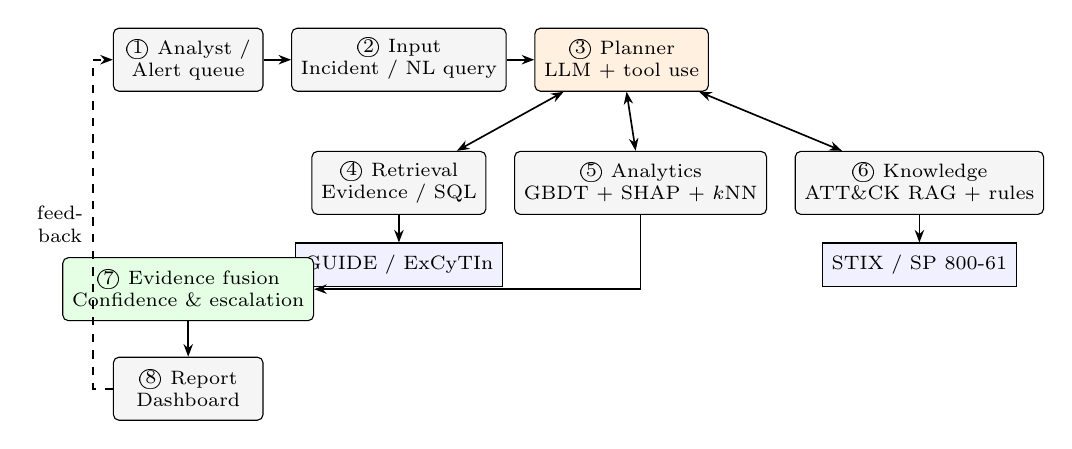
\begin{tikzpicture}[
  font=\scriptsize,
  box/.style={draw, rounded corners=2pt, align=center,
              minimum width=1.9cm, minimum height=0.8cm, fill=gray!8},
  db/.style={draw, align=center, minimum width=1.9cm,
             minimum height=0.55cm, fill=blue!6},
  arr/.style={-{Stealth[length=1.6mm]}, semithick},
  darr/.style={{Stealth[length=1.6mm]}-{Stealth[length=1.6mm]}, semithick}]
\node[box] (u) {\textcircled{1} Analyst /\\Alert queue};
\node[box, right=0.35cm of u] (q) {\textcircled{2} Input\\Incident / NL query};
\node[box, right=0.35cm of q, fill=orange!12] (p)
     {\textcircled{3} Planner\\LLM + tool use};
\node[box, below=0.75cm of q] (d) {\textcircled{4} Retrieval\\Evidence / SQL};
\node[box, right=0.35cm of d] (a) {\textcircled{5} Analytics\\GBDT + SHAP + $k$NN};
\node[box, right=0.35cm of a] (k) {\textcircled{6} Knowledge\\ATT\&CK RAG + rules};
\node[db, below=0.35cm of d] (ds) {GUIDE / ExCyTIn};
\node[db, below=0.35cm of k] (kb) {STIX / SP 800-61};
\node[box, below=2.1cm of u, fill=green!10] (r)
     {\textcircled{7} Evidence fusion\\Confidence \& escalation};
\node[box, below=0.45cm of r] (o) {\textcircled{8} Report\\Dashboard};
\draw[arr] (u) -- (q);
\draw[arr] (q) -- (p);
\draw[darr] (p) -- (d);
\draw[darr] (p) -- (a);
\draw[darr] (p) -- (k);
\draw[arr] (d) -- (ds);
\draw[arr] (k) -- (kb);
\draw[arr] (a.south) |- (r.east);
\draw[arr] (r) -- (o);
\draw[arr, dashed] (o.west) -- ++(-0.25,0) |- node[pos=0.25, left, align=center]
     {feed-\\back} (u.west);
\end{tikzpicture}
\caption{Architecture of the AI SOC Analyst Agent. The planner
(\textcircled{3}) calls retrieval, analytics, and knowledge tools; the
fusion module (\textcircled{7}) decides the label and whether to
escalate.}
\label{fig:arch}
\end{figure}

% [A2Z:PG]
Fig.~\ref{fig:arch} shows how the elements interact. The planner is
the only element that calls tools; the fusion module is the only one
that decides; and every arrow back to the analyst carries evidence
with its source.

\subsection{How the Design Goals Are Achieved}
% [A2Z:PH]
\emph{Evidence gathering under assume breach.} The planner picks the
data source by input type, widens queries along the unmet sufficiency
condition (missing account context $\rightarrow$ sign-in logs; missing
host context $\rightarrow$ process and network logs), and adds hosts
when lateral movement appears. Following~\cite{tsegai2026}, stopping is
\emph{not} left to the LLM: $\textsc{IsSufficient}(E)$ holds only if
(C1) every alert has its evidence, (C2) every principal account and
host has at least one context record, and (C3) every empty query is
confirmed not to stem from a log gap; otherwise the evidence counts as
insufficient rather than as ``no suspicious activity.'' On GUIDE, which
has no raw logs, C3 checks that evidence rows are complete and treats
placeholder entity IDs as missing.

% [A2Z:PH]
\emph{Classification.} Evidence is aggregated to incidents keyed by
(\texttt{OrgId}, \texttt{IncidentId}). Features include alert counts,
per-detector historical FP rates, entity-type distributions, and the
number of techniques and tactics; volatile indicators such as IPs and
hashes are excluded (M4). A class-weighted histogram GBDT
outputs $\mathbf{p}=(p_{TP},p_{BP},p_{FP})$, SHAP gives feature
attributions, and the $k$ nearest historical incidents are retrieved.
GBDT, not the LLM, is the classifier because GUIDE alert titles and
entity fields are anonymized IDs.

% [A2Z:PH]
\emph{Domain knowledge.} ATT\&CK STIX~2.1 objects are embedded in a
vector store for retrieval, and NIST SP~800-61 Rev.~3 and D3FEND are
distilled into playbooks. Table~\ref{tab:rules} lists the kill-chain
risk rules; later stages imply higher risk~\cite{sadlek2025,garcia2025rosca}.
The rules flag \texttt{high\_risk} and bias toward escalation but never
assign a label on their own.

\begin{table}[t]
% [A2Z:PH]
\caption{Kill-Chain Risk Rules (within One Incident)}
\label{tab:rules}
\centering
\footnotesize
\setlength{\tabcolsep}{3pt}
\begin{tabular}{@{}p{0.5cm}p{3.7cm}p{3.5cm}@{}}
\toprule
\textbf{ID} & \textbf{Condition} & \textbf{Rationale} \\
\midrule
R1 & Exfiltration or Impact tactic, or category Ransomware
   & Data may be lost or systems damaged \\
R2 & Credential Access and Lateral Movement
   & Attacker holds credentials and spreads \\
R3 & Initial Access with Execution, Persistence, or Privilege
     Escalation (any order; timestamps are noised)
   & Intrusion reached host control \\
R4 & T1070 Indicator Removal
   & Log deletion voids ``no records'' (M1) \\
R5 & $\geq 4$ distinct tactics
   & False alarms rarely span many stages \\
\bottomrule
\end{tabular}
\end{table}

\subsection{Fusion and Escalation Algorithms}
% [A2Z:PI]
Algorithm~\ref{alg:agent} is the end-to-end procedure and
Algorithm~\ref{alg:fuse} the fusion step. Because self-reported numeric
confidence from LLMs is unreliable, the LLM reports a low, medium, or
high level mapped to $c\in\{0.5,0.7,0.9\}$; its label receives $c$ and
the other two classes share $1-c$, giving $\mathbf{q}$. The fused score
is
\begin{equation}
\mathbf{s} = w_{ml}\,\mathbf{p} + w_{llm}\,\mathbf{q},\qquad
w_{ml}+w_{llm}=1,
\label{eq:fuse}
\end{equation}
with $\hat{y}=\arg\max\mathbf{s}$ and $\mathit{conf}=\max\mathbf{s}$.
An incident is auto-triaged if and only if
\begin{equation}
\mathit{conf}\ge\tau \;\wedge\; \neg\mathit{conflict} \;\wedge\;
\neg\mathit{high\_risk} \;\wedge\; \textsc{IsSufficient}(E),
\label{eq:esc}
\end{equation}
and is otherwise marked \texttt{NEEDS\_HUMAN\_REVIEW} with its reasons.
If a risk rule fires and $p_{TP}\ge\tau_{safety}$, the label is raised
to TP (M3).

\begin{algorithm}[t]
% [A2Z:PI]
\caption{SOC Triage Agent}
\label{alg:agent}
\footnotesize
\begin{algorithmic}[1]
\Require Request $Q$; model $M$; knowledge base $KB$; playbooks $PB$;
threshold $\tau$; tool budget $B$
\Ensure Triage report $R$
\State $req \gets \textsc{ValidateAndParse}(Q)$
\If{$req$ is invalid} \Return \textsc{ErrorReport}() \EndIf
\State $plan \gets \textsc{Planner.Decompose}(req)$
\State $E \gets \emptyset$;\; $calls \gets 0$
\Repeat \Comment{evidence-gathering loop}
  \State $tool \gets \textsc{Planner.SelectTool}(plan, E)$
  \State $E \gets E \cup tool.\textsc{Execute}(req, E)$ \Comment{with sources}
  \State $calls \gets calls + 1$
\Until{$\textsc{IsSufficient}(E)$ \textbf{or} $calls \ge B$}
\State $\mathbf{x} \gets \textsc{ExtractFeatures}(E)$
\State $\mathbf{p} \gets M.\textsc{PredictProba}(\mathbf{x})$;\;
       $\boldsymbol{\phi} \gets \textsc{SHAP}(M,\mathbf{x})$
\State $S \gets \textsc{SimilarIncidents}(\mathbf{x}, k)$
\State $T \gets \textsc{MapToATTACK}(E, KB)$
\State $K \gets KB.\textsc{Retrieve}(T) \cup PB.\textsc{Retrieve}(T)$
\State $llm \gets \textsc{LLM.Reason}(E,\mathbf{p},\boldsymbol{\phi},S,T,K)$
\State $(\hat{y}, conf, F) \gets \textsc{FuseEvidence}(\mathbf{p}, llm, \textsc{Rules}(T))$
\If{$conf<\tau$ \textbf{or} $\{\textit{conflict},\textit{high\_risk}\}\cap F\neq\emptyset$
    \textbf{or} \textbf{not} $\textsc{IsSufficient}(E)$}
  \State $R.status \gets$ \texttt{NEEDS\_HUMAN\_REVIEW}
\Else
  \State $R.status \gets$ \texttt{AUTO\_TRIAGED}
\EndIf
\State $R.actions \gets PB.\textsc{Recommend}(\hat{y}, T)$
\State \Return $R \cup \{\hat{y}, conf, E, \boldsymbol{\phi}, S, T, llm.rationale, F\}$
\end{algorithmic}
\end{algorithm}

\begin{algorithm}[t]
% [A2Z:PI]
\caption{FuseEvidence}
\label{alg:fuse}
\footnotesize
\begin{algorithmic}[1]
\Require ML probabilities $\mathbf{p}$; LLM output $llm$; rule results
$U$; weights $w_{ml}, w_{llm}$; safety threshold $\tau_{safety}$
\Ensure Label $\hat{y}$, confidence $conf$, flag set $F$
\State $F \gets \emptyset$
\State $\mathbf{q} \gets \textsc{OneHotWithConfidence}(llm.label, llm.level)$
\State $\mathbf{s} \gets w_{ml}\mathbf{p} + w_{llm}\mathbf{q}$
\State $\hat{y} \gets \arg\max \mathbf{s}$;\; $conf \gets \max \mathbf{s}$
\If{$\arg\max \mathbf{p} \neq llm.label$} $F \gets F \cup \{\textit{conflict}\}$ \EndIf
\If{$U$ contains a high-risk pattern}
  \State $F \gets F \cup \{\textit{high\_risk}\}$
  \If{$\hat{y}\neq \mathrm{TP}$ \textbf{and} $p_{TP} \ge \tau_{safety}$}
     $\hat{y} \gets \mathrm{TP}$ \EndIf
\EndIf
\State \Return $(\hat{y}, conf, F)$
\end{algorithmic}
\end{algorithm}

\subsection{Illustrative Example}
% [A2Z:PJ]
Consider an incident with six alerts and 20 evidence rows over two
accounts and one host (illustrative values, not experimental results).
The GBDT outputs $\mathbf{p}=(0.46,0.45,0.09)$, a near tie between TP
and BP, with the historical label rates of its detectors and alert
titles as the top SHAP features. The alerts map to Credential Access and Lateral Movement. The
LLM judges TP with medium confidence, $\mathbf{q}=(0.70,0.15,0.15)$, but
notes missing sign-in records for one account. With
$w_{ml}=w_{llm}=0.5$, (\ref{eq:fuse}) gives $\mathbf{s}=(0.58,0.30,0.12)$.
Because $\mathit{conf}=0.58<\tau$, R2 fires, and C2 is unmet,
(\ref{eq:esc}) fails and the incident is escalated with all three
reasons and a recommendation to reset credentials and inspect
lateral-movement targets.

\subsection{Key Points and Evaluation Roadmap}
% [A2Z:PK]
The key points of the design are: probabilities come from a model
trained on real labels; domain knowledge acts as a constraint, not a
suggestion; stopping and escalation are rules that can be audited; and
every conclusion carries its evidence.
% [A2Z:PL]
Section~\ref{sec:exp} evaluates these points by comparing the agent
with single-method baselines, sweeping $\tau$ to trace the
miss-rate--escalation trade-off, and ablating the classifier, the
knowledge module, and the escalation rules.

\subsection{Analytical Properties}
% [A2Z:PM]
Fix the model, weights, rules, and budget, so that for each incident
$i$ in a set $D$ the values $\hat{y}_i$, $\mathit{conf}_i$, $F_i$, and
$\textsc{IsSufficient}(E_i)$ do not depend on $\tau$. Let $A(\tau)$ be
the set of incidents satisfying (\ref{eq:esc}), let $P\subseteq D$ be
the true TP incidents, and define the TP miss rate
$\mathrm{MR}(\tau)=|\{i\in P\cap A(\tau):\hat{y}_i\neq\mathrm{TP}\}|/|P|$
and the escalation rate $\mathrm{ER}(\tau)=1-|A(\tau)|/|D|$.

\begin{proposition}\label{prop:mono}
If $\tau_1\le\tau_2$, then $\mathrm{MR}(\tau_2)\le\mathrm{MR}(\tau_1)$
and $\mathrm{ER}(\tau_2)\ge\mathrm{ER}(\tau_1)$.
\end{proposition}
\begin{IEEEproof}
Every term in (\ref{eq:esc}) except $\mathit{conf}_i\ge\tau$ is
independent of $\tau$, and $\mathit{conf}_i\ge\tau_2$ implies
$\mathit{conf}_i\ge\tau_1$. Hence $A(\tau_2)\subseteq A(\tau_1)$. The
numerator of $\mathrm{MR}$ counts a subset of $A(\tau)$ defined by a
$\tau$-independent condition, so it cannot grow when $A(\tau)$ shrinks,
and $|A(\tau_2)|\le|A(\tau_1)|$ gives the claim for $\mathrm{ER}$.
\end{IEEEproof}

\begin{proposition}\label{prop:safe}
For every $\tau$, no incident that triggers a risk rule R1--R5 is
auto-triaged; hence no TP that triggers a risk rule contributes to
$\mathrm{MR}(\tau)$.
\end{proposition}
\begin{IEEEproof}
If a rule fires, Algorithm~\ref{alg:fuse} adds $\mathit{high\_risk}$
to $F_i$, so the term $\neg\mathit{high\_risk}$ in (\ref{eq:esc}) is
false and $i\notin A(\tau)$. The numerator of $\mathrm{MR}(\tau)$ only
counts incidents in $A(\tau)$.
\end{IEEEproof}

% [A2Z:PM]
Proposition~\ref{prop:mono} makes $\tau$ a single knob that trades
analyst workload for safety, and Proposition~\ref{prop:safe}
guarantees that the cost of a missed late-stage attack is never paid
for automation.

% =====================================================================
%  IV. EXPERIMENT (Q--V)
% =====================================================================
\section{Experiment}\label{sec:exp}

\subsection{Experiments and Metrics}
% [A2Z:Q]
Table~\ref{tab:exp} lists the five experiments and the ablation. The
primary metrics are the TP miss rate $\mathrm{MR}$ and the escalation
rate $\mathrm{ER}$ defined in Section~\ref{sec:design}; we also report
macro-F1, per-class precision and recall, technique- and tactic-level
precision and recall for ATT\&CK mapping, rubric scores for report
quality (correctness, evidence completeness, actionability; human and
LLM-as-judge), and tokens, latency, and tool calls per incident.
Because LLM calls are costly, LLM-dependent experiments use stratified
samples of 1{,}000 incidents; five such runs cost at most about
US\$550 at the per-alert cost reported in~\cite{tsegai2026}.

\begin{table}[t]
% [A2Z:Q]
\caption{Experimental Design}
\label{tab:exp}
\centering
\footnotesize
\setlength{\tabcolsep}{2.5pt}
\begin{tabular}{@{}p{1.3cm}p{1.6cm}p{2.2cm}p{2.6cm}@{}}
\toprule
\textbf{Exp.} & \textbf{Data} & \textbf{Comparison} & \textbf{Metrics} \\
\midrule
E1 Triage & GUIDE & Baselines (i)--(iv) & Macro-F1, P/R, MR, ER \\
E2 ATT\&CK & GUIDE (annotated) & LLM vs.\ LLM+RAG & Technique/tactic P, R \\
E3 Investigation & ExCyTIn-Bench & Published scores; single-turn LLM & Benchmark reward \\
E4 Report & 50 sampled incidents & Without RAG & Rubric scores \\
E5 Cost & E1, E3 & -- & Tokens, latency, tool calls \\
Ablation & GUIDE & Remove \textcircled{5}, \textcircled{6}, or escalation rules & As E1 \\
\bottomrule
\end{tabular}
\end{table}

\subsection{Compared Methods}
% [A2Z:R]
E1 compares the agent with (i) majority class, (ii) a per-detector
historical-FP-rate rule, (iii) GBDT only, and (iv) LLM only without the
knowledge base. E2 compares LLM mapping with and without retrieval, E3
compares against published ExCyTIn-Bench scores and a single-turn LLM
without planning, and the ablation removes the classifier
(\textcircled{5}), the knowledge module (\textcircled{6}), or the
escalation rules in turn.

\subsection{Setup}
% [A2Z:S]
\textbf{Microsoft GUIDE}~\cite{freitas2024cgr} (CDLA-2.0) has about 13
million evidence rows, 1.6 million alerts, and 1 million incidents from
6.1k organizations. Table~\ref{tab:guide} summarizes our own profile of
the training file. \texttt{MitreTechniques} is filled in only 42.5\% of
rows, so E2 uses annotated alerts only, and remediation labels are
99.4\% missing, so recommendations are judged by rubric in E4.
\textbf{ExCyTIn-Bench}~\cite{wu2025excytin} provides 57 log tables,
eight attack chains, and 7{,}542 questions for E3.

\begin{table}[t]
% [A2Z:S]
\caption{Measured Profile of GUIDE\_Train}
\label{tab:guide}
\centering
\footnotesize
\begin{tabular}{@{}ll@{}}
\toprule
\textbf{Item} & \textbf{Value} \\
\midrule
Rows (evidence entities) & 9{,}516{,}837 \\
Incidents (\texttt{OrgId}+\texttt{IncidentId}) & 707{,}108 \\
Organizations & 5{,}769 \\
TP / BP / FP incidents & 20.6\% / 49.0\% / 30.4\% \\
Distinct ATT\&CK techniques & 432 \\
Rows with \texttt{MitreTechniques} & 42.5\% \\
Anonymized fields & AlertTitle, DetectorId, all entities \\
\bottomrule
\end{tabular}
\end{table}

% [A2Z:S]
Random row-level splits would leak alerts of one incident, or incidents
of one organization, across train and test~\cite{arp2022}. We split by
(\texttt{OrgId}, \texttt{IncidentId}): the official GUIDE test set
(303{,}220 labeled incidents) shares no incident key with the training
set, so it serves as the incident-split test set, with 10\% of the
training incidents held out for validation. We also report
organization-held-out and time-ordered splits. The agent is implemented
in Python with pandas and DuckDB, scikit-learn's histogram GBDT and SHAP,
mitreattack-python and Chroma, a tool-using LLM API, and a Streamlit
dashboard; all scripts fix random seeds.

\subsection{Parameter Tuning}
% [A2Z:T]
All parameters are tuned on the validation split only. We search
$w_{ml}\in\{0.5,0.6,0.7,0.8\}$, $\tau_{safety}\in\{0.2,0.3,0.4\}$, the
tool budget $B\in\{5,10,15\}$, the R5 tactic threshold in $\{3,4,5\}$,
and the LLM confidence mapping around $\{0.5,0.7,0.9\}$. The threshold
$\tau$ is swept over $[0.50,0.95]$ in steps of 0.05; by
Proposition~\ref{prop:mono} this traces a monotone
$\mathrm{MR}$--$\mathrm{ER}$ curve, and we select the lowest-MR point
whose ER stays within an escalation budget set with analysts.

\subsection{Results}
% [A2Z:U]
Table~\ref{tab:e1} reports E1 on the incident split, and
Fig.~\ref{fig:mr-er} shows the MR--ER trade-off obtained by sweeping
$\tau$. Without escalation, the GBDT reaches a macro-F1 of 0.780 and
misses 25.3\% of TP incidents, against 57.9\% for the detector rule.
Generalization to unseen organizations is much harder: on the
organization split the GBDT macro-F1 drops to 0.477 (detector rule
0.426), while the time split stays close to the incident split (0.765).
SHAP on 6{,}000 class-balanced test incidents shows that 75\% of the
GBDT's attribution mass comes from the historical label rates of
detectors and alert titles, whereas kill-chain features such as tactic
count and furthest stage rank only 29th--34th of 81 features. The
model thus judges similarity to past incidents rather than attack-chain
position, which is why the risk rules of Table~\ref{tab:rules} act
outside it. Among five nearest training incidents, 74\% share the true
label of the queried incident.
\TBD{} Describe the MR--ER curve, E2 precision and recall, E3 reward,
E4 rubric scores, E5 cost, and the ablation, using values from
\texttt{experiments/results/} only.

\begin{figure}[t]
% [A2Z:U]
% Placeholder: replace the [TBD] note with the measured curve
% (one point per tau in [0.50, 0.95]) once E1 has been run.
\centering
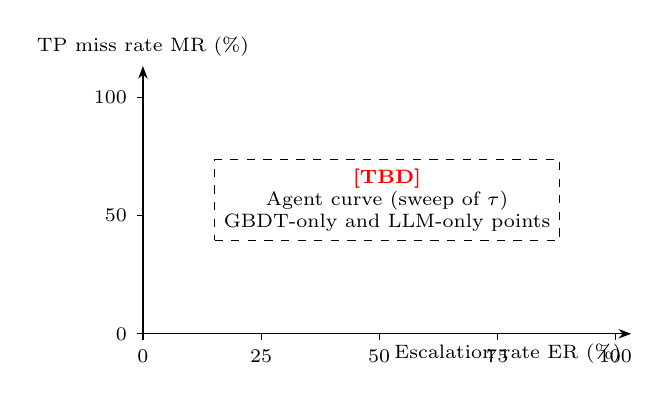
\begin{tikzpicture}[font=\scriptsize]
\draw[-{Stealth[length=1.6mm]}] (0,0) -- (6.2,0)
  node[below left, align=right] {Escalation rate ER (\%)};
\draw[-{Stealth[length=1.6mm]}] (0,0) -- (0,3.4)
  node[above, align=center] {TP miss rate MR (\%)};
\foreach \x/\l in {0/0,1.5/25,3/50,4.5/75,6/100}
  \draw (\x,0) -- (\x,-0.08) node[below] {\l};
\foreach \y/\l in {0/0,1.5/50,3/100}
  \draw (0,\y) -- (-0.08,\y) node[left] {\l};
\node[draw, dashed, align=center, fill=white] at (3.1,1.7)
  {\TBD{}\\ Agent curve (sweep of $\tau$)\\ GBDT-only and LLM-only points};
\end{tikzpicture}
\caption{TP miss rate versus escalation rate on GUIDE (incident split)
as the confidence threshold $\tau$ varies. By
Proposition~\ref{prop:mono}, raising $\tau$ moves the operating point
toward higher ER and never increases MR.}
\label{fig:mr-er}
\end{figure}

\begin{table}[t]
% [A2Z:U]
\caption{Triage Results on GUIDE (Incident Split)}
\label{tab:e1}
\centering
\footnotesize
\setlength{\tabcolsep}{3pt}
\begin{tabular}{@{}lcccc@{}}
\toprule
\textbf{Method} & \textbf{Macro-F1} & \textbf{TP recall}
& \textbf{MR} & \textbf{ER} \\
\midrule
% Values: experiments/results/e1_results.json (incident split; GBDT = mean of 3 seeds, std <= 0.001)
Majority class        & 0.219 & 0.000 & 1.000 & -- \\
Detector FP-rate rule & 0.675 & 0.421 & 0.579 & -- \\
GBDT only             & 0.780 & 0.747 & 0.253 & -- \\
LLM only (no KB)      & \TBD & \TBD & \TBD & -- \\
\textbf{Proposed agent} & \TBD & \TBD & \TBD & \TBD \\
\bottomrule
\end{tabular}
\end{table}

\subsection{Verification and Threats to Validity}
% [A2Z:V]
\TBD{} State whether the agent lowers MR relative to GBDT-only and
LLM-only at the selected ER, which module the ablation shows matters
most, and on which incidents it still fails.

% [A2Z:V]
Several threats qualify these results. GUIDE is anonymized and comes
from one vendor ecosystem, which limits LLM semantic reasoning and
generalization; ExCyTIn-Bench and organization-held-out splits
partially address this. LLMs may hallucinate mappings or actions;
retrieval with citations, cross-checking with the ML output, and
escalation on conflict reduce but do not remove this risk. Rubric
scores in E4 are partly subjective. Finally, an adversary may delete
logs to induce early closure; R4 and condition C3 treat such gaps as
signals rather than as evidence of benignity.

% =====================================================================
%  V. CONCLUSION (W--Z)
% =====================================================================
\section{Conclusion}\label{sec:concl}

% [A2Z:W]
SOC triage is overwhelmed by alerts, and neither ML classifiers nor
LLM agents alone know when a decision should go to a human. This paper
proposed the AI SOC Analyst Agent, which fuses ML probabilities,
ATT\&CK and kill-chain knowledge, and LLM reasoning, and escalates by
explicit rules.

% [A2Z:X]
The design excels where alert volume is high, evidence is incomplete,
and attacks progress through several stages: rule-based sufficiency
prevents premature closure, risk rules guarantee that late-stage
incidents reach an analyst (Proposition~\ref{prop:safe}), and a single
threshold controls the workload--safety trade-off
(Proposition~\ref{prop:mono}).

% [A2Z:Y]
\TBD{} Summarize the measured MR, ER, macro-F1, ATT\&CK mapping, and
cost results reported in Section~\ref{sec:exp}.

% [A2Z:Z]
In conclusion, turning SOC domain principles into checkable decision
rules lets an AI agent automate the routine while keeping humans in
charge of the hard cases. The main limitations are the anonymized,
single-vendor training data and the residual risk of LLM errors. Future
work will (1) add queue prioritization, (2) extend the knowledge base
to ATT\&CK for ICS for industrial IoT, and (3) study analyst trust and
complacency in a live SOC deployment.

% =====================================================================
\begin{thebibliography}{00}

\bibitem{nsb2026} National Security Bureau, ``Analysis of the PRC's
cyber threats against Taiwan's critical infrastructure in 2025,''
Taipei, Taiwan, Jan. 2026 (in Chinese).

\bibitem{mtrends2026} Google Cloud/Mandiant, ``M-Trends 2026: Data,
insights, and strategies from the frontlines,'' 2026.

\bibitem{ibm2026} IBM Security, ``Cost of a data breach report 2026,''
IBM, 2026.

\bibitem{alahmadi2022} B. A. Alahmadi, L. Axon, and I. Martinovic,
``99\% false positives: A qualitative study of SOC analysts'
perspectives on security alarms,'' in \emph{Proc. 31st USENIX Security
Symp.}, 2022, pp. 2783--2800.

\bibitem{strom2018} B. E. Strom, A. Applebaum, D. P. Miller,
K. C. Nickels, A. G. Pennington, and C. B. Thomas, ``MITRE ATT\&CK:
Design and philosophy,'' The MITRE Corporation, Tech. Rep., Jul. 2018
(revised Mar. 2020).

\bibitem{nist80061r3} NIST, ``Incident response recommendations and
considerations for cybersecurity risk management: A CSF 2.0 community
profile,'' NIST SP 800-61 Rev. 3, Apr. 2025,
doi: 10.6028/NIST.SP.800-61r3.

\bibitem{freitas2026aip} S. Freitas, A. Gharib, and M. Magenheim,
``Adaptive incident prioritization for security operations at scale,''
arXiv:2607.16963, 2026.

\bibitem{ndichu2026} S. Ndichu, T. Ban, S. Ozawa, T. Takahashi, and
D. Inoue, ``AI-driven security alert screening and alert fatigue
mitigation in security operations centers: A survey,''
arXiv:2605.08316, 2026.

\bibitem{habibzadeh2025} A. Habibzadeh, F. Feyzi, and R. Ebrahimi
Atani, ``Large language models for security operations centers: A
comprehensive survey,'' arXiv:2509.10858, 2025.

\bibitem{tsegai2026} S. A. Tsegai, A. Kantchelian, D. Yao, and P. Gao,
``From investigation failures to reliable SOC agents: Understanding and
improving LLM-based alert triage,'' arXiv:2610.10608, 2026.

\bibitem{wu2025excytin} Y. Wu \emph{et al.}, ``ExCyTIn-Bench:
Evaluating LLM agents on cyber threat investigation,'' in \emph{Proc.
Int. Conf. Mach. Learn. (ICML)}, 2026; arXiv:2507.14201.

\bibitem{tilbury2026} J. Tilbury and S. V. Flowerday, ``The vigilance
paradox: Automation reliance inside the modern SOC,'' \emph{Inf.
Comput. Secur.}, vol. 34, no. 4, pp. 639--662, 2026,
doi: 10.1108/ICS-08-2025-0318.

\bibitem{freitas2024cgr} S. Freitas, J. Kalajdjieski, A. Gharib, and
R. McCann, ``AI-driven guided response for security operation centers
with Microsoft Copilot for Security,'' arXiv:2407.09017, 2024.

\bibitem{sadlek2025} L. Sadlek, M. M. Yamin, P. \v{C}eleda, and
B. Katt, ``Severity-based triage of cybersecurity incidents using kill
chain attack graphs,'' \emph{J. Inf. Secur. Appl.}, vol. 89, 2025,
doi: 10.1016/j.jisa.2024.103956.

\bibitem{garcia2025rosca} R. Garcia, A. Lahmadi, P.-F. Gimenez, and
C. Sala, ``ROSCA: Robust and scalable security alert correlation and
prioritisation using the MITRE ATT\&CK framework,'' in \emph{Proc.
Workshop Analytics, Telemetry, and Cybersecurity for HPCC (WATCH '25)},
Taipei, Taiwan, Oct. 2025, pp. 30--37, doi: 10.1145/3733826.3762680.

\bibitem{lekssays2025} A. Lekssays, U. Shukla, H. T. Sencar, and
M. R. Parvez, ``TechniqueRAG: Retrieval augmented generation for
adversarial technique annotation in cyber threat intelligence text,''
in \emph{Findings Assoc. Comput. Linguist. (ACL)}, 2025.

\bibitem{wei2025cortex} B. Wei, Y. S. Tay, H. Liu, J. Pan, K. Luo,
Z. Zhu, and C. Jordan, ``CORTEX: Collaborative LLM agents for
high-stakes alert triage,'' arXiv:2510.00311, 2025.

\bibitem{kersten2025} L. Kersten, K. Beelen, E. Zambon, C. Snijders,
and L. Allodi, ``A field study to uncover and a tool to support the
alert investigation process of Tier-1 analysts,'' in \emph{Proc. Symp.
Usable Secur. Privacy (USEC)}, 2025, doi: 10.14722/usec.2025.23034.

\bibitem{banstola2026} K. Banstola, F. Al Faisal \emph{et al.}, ``It is
not yet another tool: Creating and deploying an agentic AI companion in
a security operations center,'' arXiv:2609.06250, 2026.

\bibitem{bianco2013} D. J. Bianco, ``The pyramid of pain,'' Mar. 2013
(updated Jan. 2014). [Online]. Available:
https://detect-respond.blogspot.com/2013/03/the-pyramid-of-pain.html

\bibitem{deason2025} L. Deason \emph{et al.}, ``CyberSOCEval:
Benchmarking LLMs capabilities for malware analysis and threat
intelligence reasoning,'' arXiv:2509.20166, 2025.

\bibitem{arp2022} D. Arp \emph{et al.}, ``Dos and don'ts of machine
learning in computer security,'' in \emph{Proc. 31st USENIX Security
Symp.}, 2022, pp. 3971--3988.

\bibitem{engelen2021} G. Engelen, V. Rimmer, and W. Joosen,
``Troubleshooting an intrusion detection dataset: The CICIDS2017 case
study,'' in \emph{Proc. IEEE Secur. Privacy Workshops (SPW)}, 2021,
pp. 7--12, doi: 10.1109/SPW53761.2021.00009.

\bibitem{yao2023react} S. Yao, J. Zhao, D. Yu, N. Du, I. Shafran,
K. Narasimhan, and Y. Cao, ``ReAct: Synergizing reasoning and acting in
language models,'' in \emph{Proc. Int. Conf. Learn. Represent.
(ICLR)}, 2023.

\end{thebibliography}

\end{document}
